% !TEX TS-program = pdflatex
% !TEX encoding = UTF-8 Unicode

% This is a simple template for a LaTeX document using the "article" class.
% See "book", "report", "letter" for other types of document.

\documentclass[11pt]{article} % use larger type; default would be 10pt

\usepackage[utf8]{inputenc} % set input encoding (not needed with XeLaTeX)

%%% Examples of Article customizations
% These packages are optional, depending whether you want the features they provide.
% See the LaTeX Companion or other references for full information.

%%% PAGE DIMENSIONS
\usepackage{geometry} % to change the page dimensions
\geometry{a4paper} % or letterpaper (US) or a5paper or....
% \geometry{margin=2in} % for example, change the margins to 2 inches all round
% \geometry{landscape} % set up the page for landscape
%   read geometry.pdf for detailed page layout information

\usepackage{graphicx} % support the \includegraphics command and options

% \usepackage[parfill]{parskip} % Activate to begin paragraphs with an empty line rather than an indent

%%% PACKAGES
\usepackage{booktabs} % for much better looking tables
\usepackage{array} % for better arrays (eg matrices) in maths
\usepackage{paralist} % very flexible & customisable lists (eg. enumerate/itemize, etc.)
\usepackage{verbatim} % adds environment for commenting out blocks of text & for better verbatim
\usepackage{subfig} % make it possible to include more than one captioned figure/table in a single float
\usepackage{graphicx}
% These packages are all incorporated in the memoir class to one degree or another...

%%% HEADERS & FOOTERS
\usepackage{fancyhdr} % This should be set AFTER setting up the page geometry
\pagestyle{fancy} % options: empty , plain , fancy
\renewcommand{\headrulewidth}{0pt} % customise the layout...
\lhead{}\chead{}\rhead{}
\lfoot{}\cfoot{\thepage}\rfoot{}

%%% SECTION TITLE APPEARANCE
\usepackage{sectsty}
\allsectionsfont{\sffamily\mdseries\upshape} % (See the fntguide.pdf for font help)
% (This matches ConTeXt defaults)

%%% ToC (table of contents) APPEARANCE
\usepackage[nottoc,notlof,notlot]{tocbibind} % Put the bibliography in the ToC
\usepackage[titles,subfigure]{tocloft} % Alter the style of the Table of Contents
\renewcommand{\cftsecfont}{\rmfamily\mdseries\upshape}
\renewcommand{\cftsecpagefont}{\rmfamily\mdseries\upshape} % No bold!
\usepackage{hyperref}
%%% END Article customizations

%%% The "real" document content comes below...

\title{Projet programmation concurrente \\
	Polytech'Nice Sophia - SI4 G1}
\author{David BORRY\\
		Thomas GILLOT}
%\date{} % Activate to display a given date or no date (if empty),
         % otherwise the current date is printed 

\begin{document}
\maketitle

Nous déclarons sur l'honneur que ce rapport et l'application qu'il décrit sont le fruit de notre propre travail, basé sur notre expérience scolaire et personnelle sur ces dernières années et que nous n'avons ni contrefait, ni falsifié, ni copié partiellement sur l'oeuvre d'autres binômes ou sur internet. Nous sommes conscients que le plagiat est considéré comme une faute grave pouvant être sévèrement sanctionnée. 

\newpage

\section{Introduction}
Ce rapport a pour sujet la conception et le développement d'une simulation de déplacement d'une foule d'individus dans un environnement comprenant plusieurs obstacles, basée sur les notions vues en cours et en TD de programmation concurrente.  \\
L'application a été écrite en C++ et utilise la bibliothèque POSIX du langage C.
Pour la représentation graphique, c'est la bibliothèque SFML qui est utilisée.
Les tests unitaires sont quant à eux réalisés avec Google Test. \\
Il n'est pas nécessaire d'avoir ces bibliothèques installées au préalable et l'application peut être compilée et éxécutée sans la partie graphique. \\
Le rapport a pour but d'expliquer le fonctionnement de l'application et les décisions prises pour la conception des principaux algorithmes,  analyser et comparer le fonctionnement des threads POSIX par rapport à Java ainsi que les performances en fonction des différentes configurations possibles



\tableofcontents

\rhead{\textbf{David BORRY - Thomas GILLOT}}

\newpage
\section{Conception}
La simulation a un objectif clair: faire converger une quantité plus ou moins grande de personnes vers une unique destination et faire en sorte qu'ils finissent tous par l'atteindre. Toutefois, elle a trois manières différentes de remplir cet objectif. La première consiste à déplacer successivement chaque personne d'une unité jusqu'à ce qu'elles aient toutes atteint leur destination. La seconde permet de gérer de la même manière ces personnes, mais en fonction de leur position dans l'une des quatre régions de tailles égales constituant le monde. Une thread est associée à chaque région. Pour la troisième technique, on crée une thread pour chaque personne à déplacer. 

\subsection{Fonctionnement général}
\subsubsection{Base du programme}
Trois scénarios bien différents peuvent donc s'appliquer, chacun ayant ses particularités en performances et en algorithmique.
Il est néanmoins important qu'elles partagent la plupart des variables et des algorithmes du programme afin qu'ils soient plus simple à maintenir et à faire évoluer. Quelque soit le scénario, on a donc toujours : 
\begin{itemize}
	
	\item L'ensemble des murs et des personnes à déplacer sur le terrain 
	\item Une destination fixée à une extrémité du terrain.
	\item Une carte du terrain constamment mise à jour où sont représentés les obstacles qu'une personne peut rencontrer (murs ou 			autres personnes).
	\item Les algorithmes permettant de créer et de déplacer d'une unité une personne en direction d'une destination donnée.
\end{itemize}

\subsubsection{Déplacement d'une personne}
Le bon fonctionnement du programme repose en grande partie sur l'algorithme de déplacement. Le programme ne se terminant que lorsqu'il n'y a plus personne à déplacer, il faut un algorithme rapide et solide prenant en compte la gestion des obstacles. Un algorithme de pathfinding pour éviter les obstacles comme \textit{Dijkstra} ou \textit{A*} serait inneficace car peu optimal avec un grand nombre de personnes à gérer et/ou une grande carte. \\
En revanche, un algorithme de type \href{https://gamedevelopment.tutsplus.com/tutorials/understanding-steering-behaviors-seek--gamedev-849}{\textit{steering behaviour}} principalement basé sur les notions de vecteurs et de distances est bien plus approprié.
L'entité à déplacer ne pourra pas éviter les obstacles de manière intelligente s'il y en a, c'est pourquoi il est possible qu'une destination fixée soit impossible à atteindre pour certaines entités (si la destination est derrière un mur et que la seule entrée pour y accéder se situe à l'autre bout du terrain, par exemple). Le choix de la destination est donc également essentiel pour que la simulation s'éxécute correctement.

\newpage

L'algorithme choisi pour la simulation fonctionne donc de cette manière : \\

Pour un \textbf{terrain}, une \textbf{entité}  et une \textbf{destination} donnés, si l'entité n'a pas atteint la destination :

\begin{itemize}
	\item soit une \textbf{queue} q.
	\item Pour chaque case \textbf{c} de \textbf{bordure}(entite)
\begin{itemize}
		\item ajouter \textbf{chemin}(c,destination) à q
	\end{itemize}

	\item tant que q  n'est pas vide:
	\begin{itemize}
		\item retirer \textbf{c} le plus petit chemin
		\item \textbf{deplacer}(entite,c)
		\item Si l'entité a bougé, arrêter.
		\item Sinon, continuer.
	\end{itemize}
	
\end{itemize}

\subsection{Gestion des threads}
Si les scénarios partagent donc la plupart des ressources du programmes, ils les utilisent tous d'une manière différente. 
Pour l'option \textbf{-t0} où la simulation est gérée par la thread principale, le fonctionnement est assez simple : tant que toutes les personnes n'ont pas atteint la destination, répéter pour chacune d'entre elles l'algorithme de déplacement décrit précédemment. On doit donc mettre à jour le monde et l'ensemble des personnes un certain nombre de fois, ce qui peut faire penser au design d'une boucle de jeu. C'est le but: de cette manière, on peut facilement intégrer la représentation graphique à la simulation en redessinant le terrain à chaque mise à jour. \\
Pour l'option \textbf{-t1}, le fonctionnement est assez semblable, mais on divise le terrain en 4 parties à gérer pour chaque thread créée. Les threads ont toujours une boucle devant déplacer des entités, mais seulement celles se trouvant dans la région associée. \\
L'option \textbf{-t2} utilise toujours une boucle, mais elle ne gère qu'une entité par thread. La boucle continue tant que l'entité n'a pas atteint sa destination.

\subsubsection{Les threads POSIX}

L'année dernière en cours d'\textbf{IHM} et de \textbf{Réseaux}, nous avons déjà eu un aperçu de la gestion des threads en \textbf{Java}. L'utilisation des threads java est plutôt orientée objet car nous les avons principalement utilisées en créant des classes héritées de \textbf{Thread}, où l'on redéfinissait la méthode \textbf{run}. Cela facilite grandement le passage de paramètres car on peut directement les mettre dans le constructeur personnalisé d'une classe fille de Thread.
Les threads java sont d'abord créés avec le constructeur et on les éxécute avec la méthode \textbf{start}. On attend la fin d'une tâche avec la méthode \textbf{join}. Les méthodes \textbf{suspend} et \textbf{resume} permettent de mettre en pause et de relancer une thread. En java, on ne peut pas détruire directement une thread. La fin de l'éxécution est en général suffisante, mais on peut s'aider de la méthode \textbf{interrupt} pour arrêter la thread en avance. \\

Les thread POSIX ont le même objectif, mais fonctionnent différemment. \\
Tout d'abord contrairement à Java, la création et l'éxécution d'une thread ne sont pas séparées et sont directement gérées par la fonction \textbf{pthread\_create}, qui prend en paramètre l'adresse d'un type \textbf{p\_thread}, une  fonction statique et un paramètre qui sera passé à cette fonction.  On ne crée donc pas de classe héritée ici et le passage de paramètres est plus délicat car la fonction statique ne peut accepter qu'un seul argument. On doit donc créer par-dessus une structure contenant les différents arguments que l'on veut mettre et on la passe en paramètre à cette fonction. On doit également utiliser la fonction \textbf{pthread\_join} pour attendre la fin d'éxécution d'une thread. Sans cela, le programme risquerait de s'arrêter avant. Il n'y a pas non plus de véritable fonction de mise en pause et de reprise comme en Java, on doit pour cela utiliser des \textbf{Mutex} et des \textbf{Signaux}.

\subsubsection{Intégrer les threads à la simulation}
Pour les deux configurations multithread, on doit faire en sorte que chaque thread puisse s'éxécuter entièrement, sans que le programme ne se termine avant. C'est rendu possible grâce aux fonctions \textbf{pthread\_create} et \textbf{pthread\_join} de la bibliothèque POSIX. Les algorithmes de gestion des threads sont donc très semblables pour les simulations t1 et t2. Ils fonctionnent de la manière suivante : 



\textbf{t1} :
\begin{itemize}
\item creer une liste \textbf{l}
\item Pour chaque region \textbf{r} du terrain :
	\begin{itemize}
		\item Créer une  thread \textbf{t}
		\item gerer\_region{r,t}
		\item ajouter r a l
	\end{itemize}

\item Pour chaque thread t de l
\begin{itemize}
		\item attendre(t)
	\end{itemize}

\end{itemize} 
 
\textbf{t2} :
\begin{itemize}
\item creer une liste \textbf{l}
\item Pour chaque entité e :
	\begin{itemize}
		\item Créer une  thread \textbf{t}
		\item gerer\_personne{e,t}
		\item  ajouter r a l
	\end{itemize}

\item Pour chaque thread t de l
\begin{itemize}
		\item attendre(t)
	\end{itemize}

\end{itemize}

\subsubsection{Synchronisation}

Plusieurs choix de synchronisations peuvent être implémentés. Le plus simple serait d'associer un moniteur ou un \textbf{mutex}, sémaphore avec un compteur de 1, à la carte entière, mais cette solution serait inefficace et reviendrait à répéter le scénario itératif de \textbf{t0} (qui n'a pas besoin de synchronisation inter-thread puisque le scénario de t0 ne contient qu'une seule thread).

\begin{itemize}
	\item \textbf {t1} \\
	Il convient d'abord de préciser le fonctionnement de la simulation t1 : On dispose de quatre \textbf{régions} représentées par des rectangles rangés de \textbf{gauche à droite}. Chaque région doit pouvoir gérer les entités qu'elle contient de manière intelligente : Parcourir la liste de toutes les entités présentes sur la carte et selectionner celles à l'intérieur de la région est coûteux et peu optimal. On préferera  associer une \textbf{liste} d'entités à chaque région. Ainsi, dés qu'une entité quitte une région, cette dernière doit la \textbf{retirer} de sa liste et l'\textbf{ajouter} à celle de la région voisine. \\

Une première synchronisation indispensable pour le bon fonctionnement du programme : Si par exemple une région ajoute et retire en même temps des entités de sa liste, certaines entités risquent d'être \textbf{perdues} et ne seront gérées, ce qui bloquerait le programme qui ne s'arrête qu'une fois que toutes les personnes ont atteint leur destination. On doit donc sécuriser l'accès aux listes avec un \textbf{mutex}, quelle que soit la version e1, e2 ou e3. \\

Comme chaque région est adjacente à une autre, certaines cases de la cartes peuvent être partagées par deux threads. Il s'agit de la "\textbf{frontière}" où les entités passent d'une région à une autre, ce qui peut perturber la gestion des collisions si on ne sécurise pas non plus l'accès à ces cases.
Lorsqu'une entité se déplace sur une frontière, les cases qu'elle occupe peuvent se trouver dans deux régions différentes. Sachant que la position d'une entité correspond à celle de la case en Nord-Ouest, elle peut être gérée par une région tout en occupant les cases d'une autre. On doit donc synchroniser l'accès à ces cases comme le montre l'illustration suivante pour que les collisions entre entités soient bien gérées partout sur la carte. 4 mutex sont ainsi utilisés pour chaque entité se déplaçant sur une frontière. On peut également gérer l'accés aux cases avec un moniteur, la variable conditionnelle étant un boléen (\textbf{pris} ou \textbf{libre}) car on doit s'assurer qu'une seule thread à la fois puisse y accéder.

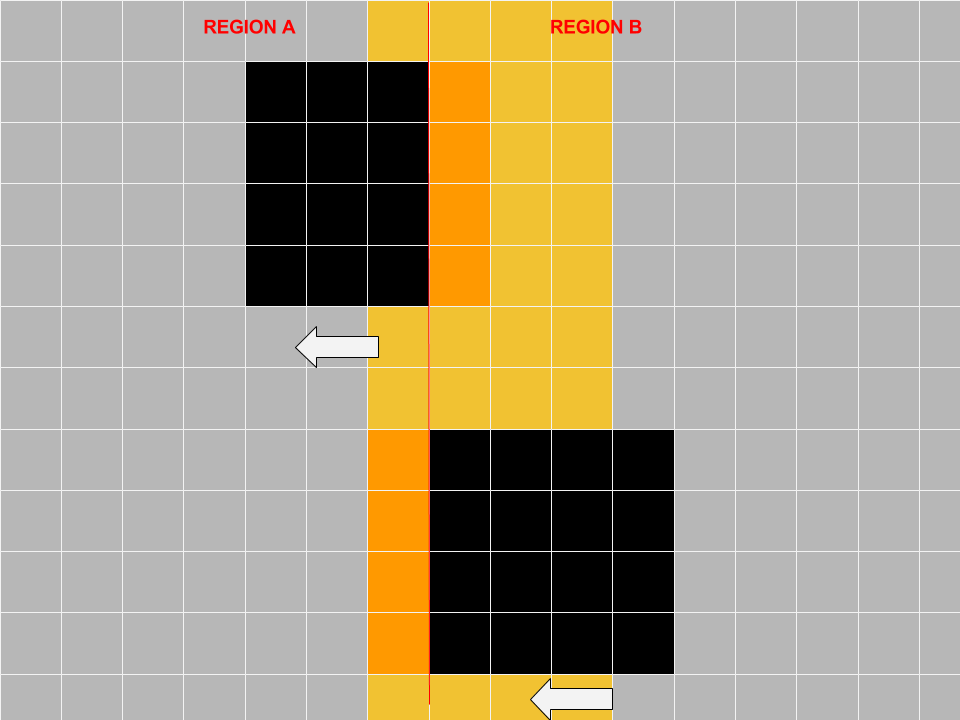
\includegraphics[scale=0.3]{synct1}




	\item \textbf {t2}

Pour t2, une solution plus optimale serait d'associer un mutex ou un moniteur à chaque case, et en fonction du scénario, seulement certaines cases devront être synchronisées. 
La synchronisation se fait au niveau du déplacement d'une entité. Quelle que soit la direction, une entité se déplaçant va essayer d'occuper 4 cases (celles vers lesquelles on se dirige) et d'en libérer 4 (celles laissées après déplacement). La synchronisation doit donc se faire au niveau des 4 cases qu'on essaie d'occuper et des 4 qu'on libère éventuellement. Avant de vérifier si elles sont occupées ou non, on attend que chacune des cases soit disponible pour éviter que deux entités aient accès à la même case. Ainsi pour chaque entité déplacée, ce sont 8 mutex (ou moniteurs) qui sont utilisés.

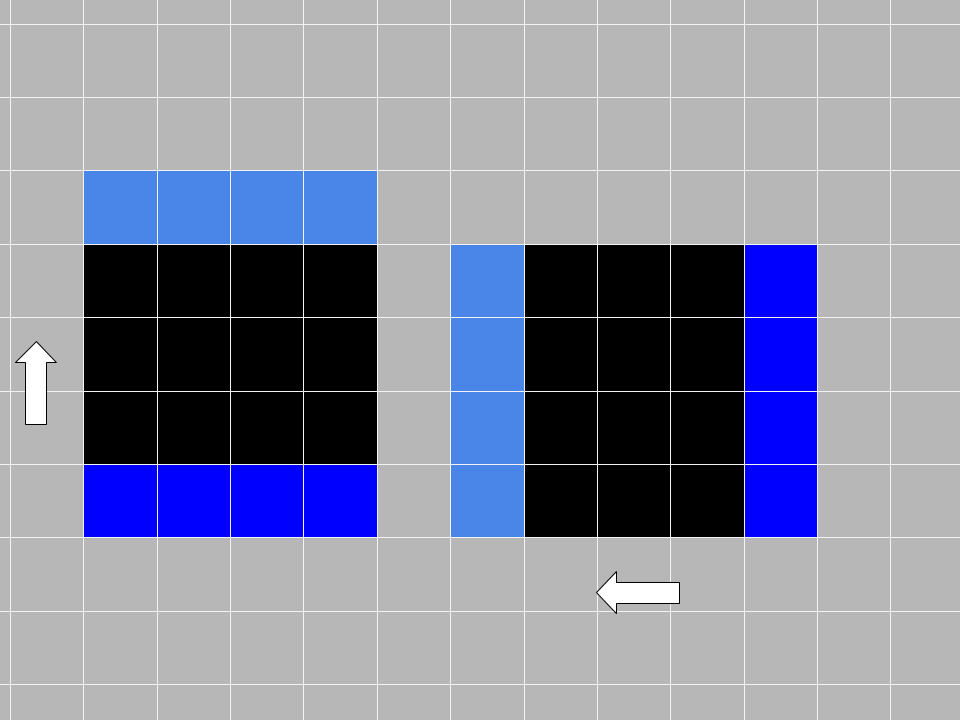
\includegraphics[scale=0.2865]{synct2}

\end {itemize}

\section{Choix de développement}
En dehors de la gestion des threads et des options entrées par l'utilisateur, le programme est principalement développé en C++ et tire parti de la programmation orientée objet, du polymorphisme et de la surcharge d'opérateurs. \\
La carte du monde est ainsi représentée par un tableau à deux dimensions contenant des cellules pouvant être \textbf{solides} (occupées par un obstacle) ou non. \\
Les vecteurs utilisés pour déplacer nos entités ont leur propre structure, \textbf{Vector2i} et peuvent être additionnés, soustraits, comparés par leur longueur et multipliés par un scalaire. Les régions du terrain à gérer pour le scénario \textbf{t1} ont également une structure \textbf{Rectangle} comprennant les points Nord-Ouest et Sud-Est de la région. \\
La classe \textbf{World} permet de gérer les déplacements d'une partie ou de la totalité des entités du terrain. Les entités à déplacer sont stockées dans une liste de pointeurs, et sont modélisées dans la plus grande classe de l'application.

\subsection{Modéliser une entité}
Il faut d'abord pouvoir définir ce qu'est une entité dans un monde représenté par un ensemble de cellules. 
Une \textbf{entité} est une forme rectangulaire composée de cellules, pouvant être solide ou non. Elle est définie par une position, une longueur, une largeur et un booléen définissant sa solidité. Elle peut également se déplacer dans toutes les directions et elle peut être détruite avant de réapparaître à sa position d'origine. \\
Une entité peut donc être une personne, un mur ou un trou. Les seules données qui changent à chaque type sont les dimensions et la solidité, c'est pourquoi il est inutile de créer une nouvelle classe fille pour chaque type. Il est préférable de stocker ces données dans un fichier (ici \textbf{DataTable}) afin de les utiliser simplement et rapidement dans le constructeur. Le reste des attributs et fonctions, en particulier celle de déplacement, ne changent pas.
 L'algorithme de déplacement cité précédemment est implémenté dans la fonction \textbf{update}. \\
Cette fonction n'est appelée que si l'entité a une destination a atteindre (\textbf{mTarget}). Grâce à la structure \textbf{Vector2i}, le calcul d'une direction à suivre est assez simple: on soustrait au vecteur destination un vecteur position donné. Pour l'entité à déplacer, cette position est basée sur les bordures, à savoir les cellules extérieures du rectangle. Ainsi, pour un humain occupant 4x4 cellules, 12 directions sont calculées. Ces directions sont ensuite stockées dans une structure de données \textbf{Priority Queue} où elles sont rangées dans l'ordre croissant. De cette manière, chaque retrait de la tête de file renverra la direction à la plus petite distance. \\

Quant au déplacement d'une case en lui-même, son implémentation est également basique: on vérifie qu'il n'y a pas d'obstacle et s'il y en a un, on peut annuler la vélocité verticale et/ou horizontale de l'entité en fonction de sa position. \\
On remarquera que la classe World dispose également d'une fonction \textbf{update}, dans laquelle on applique la fonction du même nom pour chacune des entités à déplacer. Comme il a été dit précédemment cela ressemble fortement à une boucle de jeu, facilitant ainsi l'intégration de la représentation graphique.


\subsection{Simulation et polymorphisme}
L'application en elle-même est lancée à travers les classes héritant de \textbf{Simulation}. On génère le monde et les entités dans le constructeur, et on lance la boucle dans la fonction \textbf{run}. Cette fois-ci, l'usage du polymorphisme est avantageux car cette fonction doit avoir un comportement bien différent pour chaque scénario. On crée donc des classes filles \textbf{STSim},  \textbf{MTSim1} et \textbf{MTSim2} respectivement associées aux configurations \textbf{-t0}, \textbf{-t1} et \textbf{-t2}. La fonction run est alors redéfinie pour pouvoir gérer la création des threads et l'attente de leur terminaison. La génération du monde peut également changer pour chaque classe.
Comme les threads POSIX ne peuvent pas gérer des fonctions membres directement, on recrée dans ces classes des fonctions \textbf{statiques} pour gérer les déplacements dans le monde.  \\

La classe \textbf{Entity} est également dérivée pour chaque type de synchronisation possible. Les fonctions de déplacement y sont redéfinies pour pouvoir intégrer une synchronisation au niveau de certaines cases. On peut donc lancer une simulation avec des entités simples, de type \textbf{RegionSyncEntity} pour t1 et \textbf{FullSyncEntity} pour t2. \\

Enfin, les fonctions d'accés et de sortie de section critiques doivent être redifinies si on utilise une synchronisation par mutex ou moniteur. La classe \textbf{Cell} représentant les cases de la carte est donc héritée avec la classe \textbf{MonitorCell} dans le cas où on appliquerait le scénario \textbf{e3}.

\section{Tester l'application}
Le fonctionnement de l'application repose essentiellement sur trois données: La position du point azimuth, qui doit être accessible à tout le monde, l'algorithme de déplacement et la gestion des threads. Cette dernière est uniquement nécessaire pour les configurations \textbf{t1} et \textbf{t2}.

\subsection{Correction}

Le problème du point azimuth est facile à résoudre: il ne doit pas être entouré d'obstacles et doit être situé vers la sortie du terrain. Dans cette simulation, le monde est occupé par deux murs séparés d'une certaine distance avec un trou de largeur suffisante pour qu'on puisse le traverser. Le point azimuth est fixé dans le trou du premier mur, celui de la sortie. Il est donc placé vers le milieu du mur et chaque entité finira par l'atteindre quelque soit sa position, à condition que l'algorithme de déplacement fonctionne correctement.


\begin{figure}[h]
\caption{\label{f1} \textbf{Simulation lancée avec les options -t0 et -p9}}
  \centering
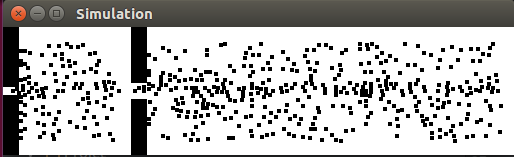
\includegraphics[width=12cm]{graph}
\end{figure}

\begin{figure}[h]
\caption{\label{f2} \textbf{La même simulation 40 itérations après}}
  \centering
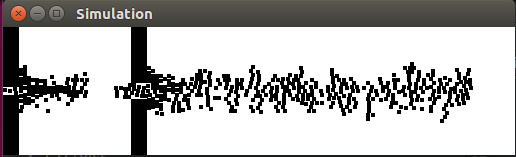
\includegraphics[width=12cm]{graph2}
\end{figure}

Les trois scénarios ont en commun le fait qu'ils utilisent des boucles pour déplacer les individus : tant que la destination n'a pas été atteinte, continuer à essayer de déplacer. La simulation ne s'arrêtera donc qu'une fois que tout le monde aura quitté le terrain. Ces scénarios fonctionnent si le point azimuth est bien placé vers la sortie, comme le montre la figure ~\ref{f2}. 
Pour vérifier l'efficacité de l'algorithme de déplacement, une série de tests unitaires doit être effectuée pour voir si le programme traite correctement le calcul des vecteurs, les directions et la gestion des obstacles. 
Le programme peut toutefois boucler à l'infini si on place volontairement le point à un endroit inatteignable.
Aussi, si la simulation fonctionne correctement pour la thread principale, ce n'est évidemment pas encore le cas pour les cas \textbf{t1} et \textbf{t2}. Les entités finissent quand même par atteindre leur destination car elles utilisent toujours le même algorithme de déplacement, mais des problèmes de collisions sont présents. 
En effet, les ressources partagées par les threads crées dans les deux cas sont la carte du terrain et la liste des entités humaines, or elles sont constamment mises à jour. Sans modèle de synchronisation implémenté, les threads peuvent se baser sur des informations faussées ou obsolètes. Une entité peut alors se déplacer sur une case non solide, mais qui parallèlement est occupée par une autre entité déplacée par une thread. Les personnes se déplacent toujours, mais en traversant certains obstacles ou en bloquant là où il n'y en a pas.

\subsection{Tests unitaires}
Les tests sont placés dans un répertoire du même nom et le projet peut être compilé sans les inclures. Aussi, \textbf{il n'est pas nécessaire d'avoir installé Google Test} pour les compiler, la bibliothèque étant directement incluse dans le projet. Il faut toutefois avoir \textbf{CMake} installé pour pouvoir compiler le CMakeLists à la racine du projet. Il y aura alors une installation complète de la simulation avec les tests inclus. \\

Pour l'instant, ils servent principalement à tester l'algorithme de déplacement qui se base sur de nombreuses parties du programme, la première et plus importante étant les vecteurs. La structure \textbf{Vector2i} et tous les opérateurs qui y sont associés sont testés dans le fichier \textbf{vector\_test.cpp}. On s'assure ainsi que le programme sait calculer correctement une direction entre deux points et une distance minimale, ce qui constitue la base de l'algorithme de déplacement. 
Les déplacements des entités sont également testés dans le fichier \textbf{entity\_test.cpp}. On doit vérifier qu'elle ne traverse pas d'obstacle et qu'elle adapte sa trajectoire si elle en rencontre un. On a pour cela plusieurs tests où l'on crée une entité sur une petite carte où on y a placé manuellement plusieurs obstacles et on analyse le comportement de l'entité. Combinés avec les vecteurs, ces tests prouvent l'efficacité de l'algorithme de déplacement. Pour que ces tests fonctionnent efficacement, les entités sont toujours placées au même endroit.

\subsection{Performances}
La simulation peut être éxécutée avec l'option \textbf{-m}, permettant d'effectuer des mesures moyennes sur le temps de réponse et de calcul du processeur. On lance ainsi la simulation 5 fois d'affilée, on effectue les mesures à chaque fois et on calcule la moyenne des trois moyennes intermédiaires à la fin. La réinitialisation de la simulation qui consiste à faire réapparaître les entités à leurs positions d'origines n'est pas incluse dans la mesure. Pour ces mesures, on met bien l'accent sur les différences entre le temps de réponse, c'est à dire le temps écoulé du point de vue d'un utilisateur, et le temps CPU consommé qui peut vite augmenter pour une application multithread. On utilise ainsi les fonctions POSIX \textbf{getrusage} et \textbf{gettimeofday} dans une classe \textbf{Measures} afin de calculer le \textbf{temps de réponse}, le \textbf{temps CPU utilisateur} et le \textbf{temps CPU système}. Les figures suivantes permettent d'analyser les temps réels et CPU pour les scénarios t0, t1 et t2 avec les trois versions. Chaque graphe a trois points correspondant aux mesures pour 4, 16 et 256 personnes. On a choisi une échelle logarithmique pour plus de visibilité.
On remarquera que pour chacune de ces mesures, le temps CPU système a une valeur négligeable.


\begin{figure}[!h]
  \centering
\caption{Comparaison des temps réels et processeurs pour t0}

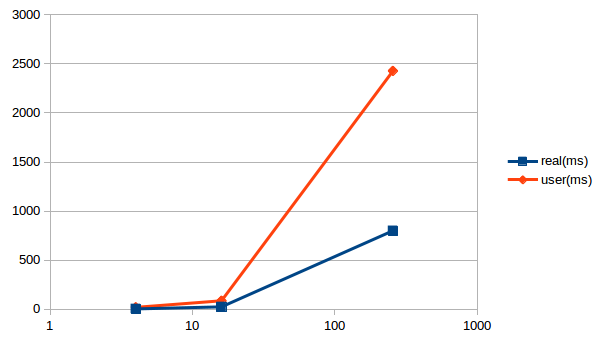
\includegraphics[width=10cm, height=4cm]{t0}

 \caption{Comparaison des temps réels et processeurs pour t1 (e1 et e2)}

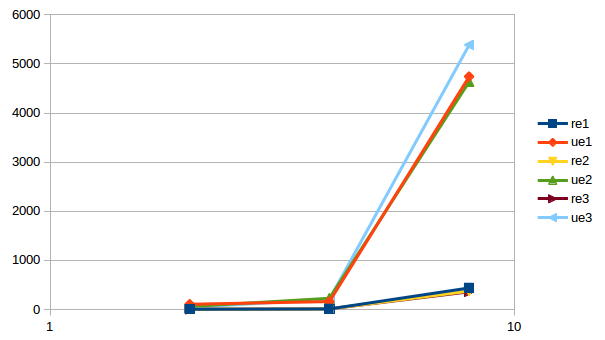
\includegraphics[width=10cm,height=4cm]{t1e3}

 \caption{Comparaison des temps réels et processeurs pour t2 (e1 et e2)}

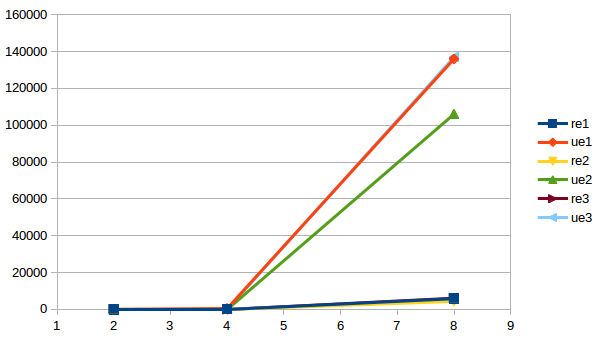
\includegraphics[width=10cm,height=4cm]{t2e3}
\end{figure}


\newpage

On peut voir que pour t0, les temps réels et utilisateurs sont assez proches avec une différence maximum de 1.5 secondes. \\
Cette différence s'accentue évidemment pour t1 et t2, avec la gestion de plusieurs threads. Plus le nombre de personne augmente, plus le temps d'éxécution est long, mais le temps CPU croit beaucoup plus vite que le temps réel. \\
Pour t1, on remarquera que les temps réels pour e1 et e2 sont identiques, mais que le temps utilisateur est plus élevé pour la première version. Même constat pour t2, avec une différence entre les deux versions encore plus grande, de l'ordre de plusieurs dizaines de secondes. On remarquera que pour t1 comme pour t2, le temps utilisateur e3 est plus élevé que celui de e2, ce qui s'explique par le fait que l'utilisation d'une variable conditionnelle augmente le nombre d'opérations élémentaires, et donc le temps CPU pour l'accés en section critique.


\section{Conclusion}
La première étape a permis de mettre en place une simulation pleinement fonctionnelle avec la thread principale et de poser les bases pour développer les scénarios multithreads. Avec la seconde, nous avons mis en place des cas simples de synchronisations des scénarios multithreads t1 et t2, que nous avons enrichis avec la troisième et dernière étape avec la synchronisation par moniteurs.
Les mesures effectuées ont bien montré l'intérêt d'un programme multithread pour ce genre de problème, qui donne un véritable gain de performances pouvant être encore amélioré avec la synchronisation des threads.
Ce projet a enfin permis pour nous d'apprendre les principes de conception d'une application multithread, les processus concurrents, le partage des ressources et les sections critiques.


\end{document}
\grid
